\documentclass[11pt]{article}

\usepackage[T1]{fontenc}
\usepackage{lmodern}
\usepackage[margin=1in]{geometry}
\usepackage{microtype}
\usepackage{amsmath,amssymb,amsthm}
\usepackage{booktabs}
\usepackage{array}
\usepackage{enumitem}
\usepackage{tikz}
\usepackage{xcolor}
\usepackage{xurl}
\usepackage[hidelinks]{hyperref}

\newtheorem{theorem}{Theorem}
\newtheorem{lemma}[theorem]{Lemma}
\newtheorem{proposition}[theorem]{Proposition}
\theoremstyle{definition}
\newtheorem{definition}[theorem]{Definition}
\theoremstyle{remark}
\newtheorem{remark}[theorem]{Remark}

\newcommand{\Q}{Q}
\newcommand{\interior}{\operatorname{int}}
\newcommand{\abs}[1]{\left|#1\right|}
\newcommand{\norminf}[1]{\left\lVert #1\right\rVert_{\infty}}

\title{An Exact Computer-Assisted Lower Bound for\\Packing 17 Unit Squares in a Square}
\author{Mira\\\small \url{https://github.com/Mira-acc/17squares}}
\date{August 2026}

\hypersetup{
  pdftitle={An Exact Computer-Assisted Lower Bound for Packing 17 Unit Squares in a Square},
  pdfauthor={Mira},
  pdfsubject={Computer-assisted discrete geometry},
  pdfkeywords={square packing, unavoidable points, computer-assisted proof, exact arithmetic}
}

\begin{document}
\maketitle

\begin{abstract}
Let $s(n)$ denote the least side length of a square that contains $n$ pairwise
interior-disjoint unit squares, with arbitrary orientations.  We prove by an
exact computer-assisted argument that
\[
  s(17) > \frac{4\,468\,292}{1\,000\,000}=4.468292.
\]
The previous exact computer-assisted bound was $s(17)>4.456575$.  Our proof
gives sixteen rational points in the square of side $4.468292$ and certifies
that every contained unit square, at every orientation, contains one of these
points strictly in its interior.  Besides direct point witnesses, the
certificate uses a strict triangle-piercing lemma to cover center regions
independently of orientation.  The result then follows by the pigeonhole
principle.  The universal geometric assertion is checked by a
$122{,}626{,}747$-node recursive bisection of the three-dimensional pose space.
All decisive comparisons are exact integer inequalities.  A fast C++ checker
and separately implemented arbitrary-precision C++ and Python checkers validate
the same certificate.
\end{abstract}

\section{Introduction}

For $L>0$, write
\[
  \Q_L=[0,L]^2.
\]
Let $s(n)$ be the minimum $L$ for which $n$ pairwise interior-disjoint unit
squares can be placed in $\Q_L$, with arbitrary translations and rotations.
The minimum is attained by the standard compactness argument: centers and
orientations range over a compact parameter space, and the containment and
nonoverlap constraints are closed.  This classical packing problem has a long
history; Friedman's dynamic survey
collects the principal constructions and lower-bound methods\cite{Friedman2009}.
For $n=17$, the survey records the lower bound
\[
  s(17)\ge \frac{40\sqrt2+19}{17}
  =4.445208382054341\ldots,
\]
attributed there to Trevor Green.  The best known construction is due to John
Bidwell and has side approximately
$4.67553009360455$\cite{Friedman2009,Ellsworth2026}.

The first exact certificate in this line proved $s(17)>4.450837$.  Fort then
optimized the rational point set within the same point-witness architecture and
proved $s(17)>4.456575$\cite{Fort2026}.  The certificate below changes the point
set again and adds an orientation-independent triangle witness.

Our result is the following.

\begin{theorem}\label{thm:main}
No packing of seventeen unit squares exists in $\Q_L$ for
\[
  L=\frac{4\,468\,292}{1\,000\,000}.
\]
Consequently,
\[
  s(17)>4.468292.
\]
\end{theorem}

The improvement over the preceding exact bound is $0.011717$.  The proof uses
the unavoidable-point method associated with
Stromquist and developed in this setting by Friedman\cite{Friedman2009,Stromquist2003}.
The new contribution is an explicit rational point set, the strict
triangle-piercing leaf described below, and an exact certificate covering the
full continuum of square positions and orientations.

\section{Strictly unavoidable points}

\begin{definition}
A finite set $P\subseteq \Q_L$ is \emph{strictly unavoidable for unit squares}
if every unit square $U\subseteq \Q_L$ satisfies
\[
  P\cap\interior(U)\ne\varnothing.
\]
\end{definition}

\begin{lemma}[Pigeonhole lemma]\label{lem:pigeonhole}
If $\Q_L$ contains a strictly unavoidable set of $n-1$ points, then no packing
of $n$ pairwise interior-disjoint unit squares exists in $\Q_L$.
\end{lemma}

\begin{proof}
Suppose $U_1,\dots,U_n$ were such a packing.  For each $i$, choose
$p_i\in P\cap\interior(U_i)$.  If $p_i=p_j$ for $i\ne j$, then that point lies
in both square interiors, contradicting interior-disjointness.  Thus the map
$i\mapsto p_i$ is an injection from an $n$-element set into an $(n-1)$-element
set, which is impossible.
\end{proof}

The use of interiors is important.  Boundary witnesses could be shared by
several touching squares and would not imply the injection in
Lemma~\ref{lem:pigeonhole}.

For Theorem~\ref{thm:main}, the set $P$ consists of the sixteen rational points
in Table~\ref{tab:points}.  Every displayed decimal is exact, with denominator
$10^7$.

\begin{table}[t]
\centering
\caption{The sixteen rational witness points.}
\label{tab:points}
\small
\setlength{\tabcolsep}{8pt}
\begin{tabular}{rcc@{\qquad}rcc}
\toprule
$i$ & $x_i$ & $y_i$ & $i$ & $x_i$ & $y_i$\\
\midrule
 1 & 0.9633740 & 0.9849850 &  9 & 0.9172158 & 2.6508741\\
 2 & 1.6317845 & 0.9829523 & 10 & 1.4694893 & 2.6410332\\
 3 & 2.5287879 & 0.9446006 & 11 & 2.4689011 & 2.6753176\\
 4 & 3.4682923 & 0.9443212 & 12 & 3.4682923 & 2.7101964\\
 5 & 0.9999997 & 1.7580956 & 13 & 0.9999997 & 3.5239708\\
 6 & 1.9993909 & 1.7929744 & 14 & 1.9395041 & 3.5236914\\
 7 & 2.9988027 & 1.8272588 & 15 & 2.8365087 & 3.4853407\\
 8 & 3.5451063 & 1.8219620 & 16 & 3.4687946 & 3.4687946\\
\bottomrule
\end{tabular}
\end{table}

\begin{figure}[t]
\centering
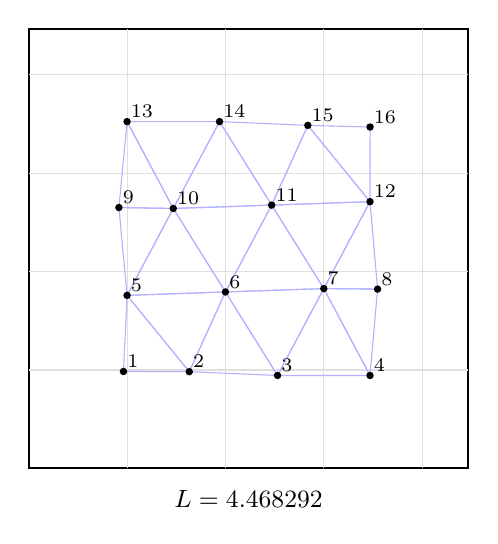
\begin{tikzpicture}[x=1.25cm,y=1.25cm]
  \draw[line width=0.7pt] (0,0) rectangle (4.468292,4.468292);
  \foreach \g in {1,2,3,4} {
    \draw[gray!25,thin] (\g,0) -- (\g,4.468292);
    \draw[gray!25,thin] (0,\g) -- (4.468292,\g);
  }
  \coordinate (p1) at (0.9633740,0.9849850);
  \coordinate (p2) at (1.6317845,0.9829523);
  \coordinate (p3) at (2.5287879,0.9446006);
  \coordinate (p4) at (3.4682923,0.9443212);
  \coordinate (p5) at (0.9999997,1.7580956);
  \coordinate (p6) at (1.9993909,1.7929744);
  \coordinate (p7) at (2.9988027,1.8272588);
  \coordinate (p8) at (3.5451063,1.8219620);
  \coordinate (p9) at (0.9172158,2.6508741);
  \coordinate (p10) at (1.4694893,2.6410332);
  \coordinate (p11) at (2.4689011,2.6753176);
  \coordinate (p12) at (3.4682923,2.7101964);
  \coordinate (p13) at (0.9999997,3.5239708);
  \coordinate (p14) at (1.9395041,3.5236914);
  \coordinate (p15) at (2.8365087,3.4853407);
  \coordinate (p16) at (3.4687946,3.4687946);
  \foreach \a/\b/\c in {
    1/2/5,2/3/6,2/5/6,3/4/7,3/6/7,4/7/8,
    5/6/10,5/9/10,6/7/11,6/10/11,7/8/12,7/11/12,
    9/10/13,10/11/14,10/13/14,11/12/15,11/14/15,12/15/16}
    \draw[blue!30,thin] (p\a) -- (p\b) -- (p\c) -- cycle;
  \foreach \x/\y/\n in {
    0.9633740/0.9849850/1,1.6317845/0.9829523/2,
    2.5287879/0.9446006/3,3.4682923/0.9443212/4,
    0.9999997/1.7580956/5,1.9993909/1.7929744/6,
    2.9988027/1.8272588/7,3.5451063/1.8219620/8,
    0.9172158/2.6508741/9,1.4694893/2.6410332/10,
    2.4689011/2.6753176/11,3.4682923/2.7101964/12,
    0.9999997/3.5239708/13,1.9395041/3.5236914/14,
    2.8365087/3.4853407/15,3.4687946/3.4687946/16}
  {
    \fill (\x,\y) circle[radius=1.35pt];
    \node[font=\scriptsize,anchor=south west,inner sep=1.2pt] at (\x,\y) {\n};
  }
  \node[font=\small,anchor=north] at (2.234146,-0.12) {$L=4.468292$};
\end{tikzpicture}
\caption{The witness set and the eighteen certified triangles.  The proof uses
the exact rational coordinates in Table~\ref{tab:points}; blue edges indicate
the orientation-independent triangle witnesses.}
\label{fig:points}
\end{figure}

\section{Parameterizing a unit square}

A unit square is unchanged by a rotation through $\pi/2$.  We may therefore
represent every orientation by an angle
\[
  -\frac{\pi}{4}\le \theta\le\frac{\pi}{4},
  \qquad t=\tan\theta\in[-1,1].
\]
Let $(x,y)$ be the center of the square, and let $p=(p_x,p_y)$ be a fixed
point.  Put
\[
  \Delta x=p_x-x,\qquad \Delta y=p_y-y,
  \qquad r=\sqrt{1+t^2}.
\]
In coordinates aligned with the square, the displacement from the center to
$p$ is
\[
  \left(\frac{\Delta x+t\Delta y}{r},
        \frac{-t\Delta x+\Delta y}{r}\right).
\]
Consequently, $p$ lies strictly inside the square exactly when
\begin{align}
  4(\Delta x+t\Delta y)^2 &< 1+t^2,\label{eq:inside-a}\\
  4(-t\Delta x+\Delta y)^2 &< 1+t^2.\label{eq:inside-b}
\end{align}

The axis-parallel half-extent of a unit square with parameter $t$ is
\[
  h(t)=\frac{1+\abs{t}}{2\sqrt{1+t^2}}.
\]
Thus containment in $\Q_L$ requires
\[
  h(t)\le x,y\le L-h(t).
\]
The function $u\mapsto(1+u)/(2\sqrt{1+u^2})$ is nondecreasing on $[0,1]$.
This monotonicity supplies a simple exact test for pose boxes that cannot
contain any feasible square.

\section{The subdivision certificate}\label{sec:certificate}

The pose space is parameterized by $(x,y,t)$.  The checker begins with the
rational box
\[
  \mathcal B_0=
  \left[\frac12,L-\frac12\right]^2\times[-1,1],
\]
which contains every feasible pose.  It recursively bisects boxes in one of
the three coordinates.  Each node is encoded by one byte:

\begin{center}
\begin{tabular}{cl}
\toprule
Byte & Meaning\\
\midrule
$0$ & the current box contains no feasible square pose;\\
$1,\dots,16$ & the indicated point lies strictly inside every pose in the box;\\
$17,18,19$ & bisect the box in $x$, $y$, or $t$, respectively.\\
$20,\dots,37$ & the indicated triangle pierces every pose in the box.\\
\bottomrule
\end{tabular}
\end{center}

The verifier distrusts every leaf claim and recomputes it from the box
endpoints.

\subsection{Infeasible leaves}

For a box
\[
  \mathcal B=[x_0,x_1]\times[y_0,y_1]\times[t_0,t_1],
\]
let
\[
  u=\min\{\abs t:t\in[t_0,t_1]\}.
\]
Since $h(t)\ge h(u)$ throughout the box, the box is infeasible if any one of
\[
  x_1<h(u),\quad L-x_0<h(u),\quad
  y_1<h(u),\quad L-y_0<h(u)
\]
holds.  The checker clears denominators and squares nonnegative quantities, so
this test is performed using integers only.

\subsection{Point-witness leaves}

Fix a witness point $p$.  Exact interval arithmetic over $\mathcal B$ gives
intervals containing
\[
  A=\Delta x+t\Delta y,
  \qquad B=-t\Delta x+\Delta y.
\]
Write $M_A$ and $M_B$ for the maximum absolute endpoint of these intervals.
Because $1+t^2\ge1+u^2$ throughout the box, the two strict inequalities
\[
  4M_A^2<1+u^2,
  \qquad 4M_B^2<1+u^2
\]
prove simultaneously that $p$ is strictly inside every square represented by
that box.  Again, the implementation stores rational endpoints on fixed grids
and clears every denominator before comparison.

The interval enclosure for the bilinear term $t\Delta y$ is obtained by taking
the minimum and maximum of its four corner products; the same is done for
$(-t)\Delta x$.  No floating-point approximation enters a leaf decision.

\subsection{Triangle-witness leaves}

Some center boxes can be closed without subdividing the orientation interval.
The certificate fixes eighteen triangles whose vertices belong to the witness
set and applies the following lemma.

\begin{lemma}[Strict triangle piercing]\label{lem:triangle}
Let $A,B,C$ be three points whose pairwise distances are strictly less than
one.  Every unit square whose center lies strictly inside triangle $ABC$
contains at least one of $A,B,C$ strictly in its interior.
\end{lemma}

\begin{proof}
Translate the square center to the origin and rotate the plane so the square is
$[-1/2,1/2]^2$.  Its diagonals divide the plane into right, top, left, and
bottom closed cones.  Because the origin lies strictly inside triangle $ABC$,
the three vertices cannot all lie in a closed half-plane bounded by either
diagonal.  Among the four cones this forces two vertices into opposite cones.
If neither vertex were in
the square interior, vertices in the right and left cones would have
$x$-coordinates differing by at least one; vertices in the top and bottom
cones would have $y$-coordinates differing by at least one.  In either case
their Euclidean distance would be at least one, contradicting the strict
side-length hypothesis.
\end{proof}

For a triangle leaf, the checker first verifies the three strict inequalities
\[
  \lVert A-B\rVert_2^2<1,\qquad
  \lVert B-C\rVert_2^2<1,\qquad
  \lVert C-A\rVert_2^2<1.
\]
It orients the triangle counterclockwise and checks that all four corners of
the center rectangle lie strictly to the left of each directed edge.  Each
edge test is affine in the center coordinates, so positivity at the four
corners proves positivity throughout the rectangle.  Lemma~\ref{lem:triangle}
then covers every orientation in the box.  The checker clears denominators and
performs these tests with integers only.

\subsection{Completeness of the tree}

The checker traverses the tree from $\mathcal B_0$, applying every split exactly.
It rejects an early end of file, an unknown opcode, a false leaf claim, or any
trailing byte.  Finally it checks the full-binary-tree identity
\[
  \#\text{leaves}=\#\text{split nodes}+1.
\]
It follows inductively that the accepted leaves form a cover of the complete
root box.  Every feasible pose is therefore covered by either a point-witness
leaf or a triangle-witness leaf.  In both cases at least one of the sixteen
points lies strictly inside the square, so the point set is strictly
unavoidable.

Lemma~\ref{lem:pigeonhole} now rules out a packing in $\Q_L$, and therefore in
every smaller container as well.  Thus $s(17)\ge L$.  The minimum defining
$s(17)$ is attained by compactness, so equality would give a packing in
$\Q_L$.  Hence $s(17)>L$, proving Theorem~\ref{thm:main}.

\section{Exact arithmetic and reproducibility}

The certificate uses the scales
\[
  S_t=2^{40},\qquad S_x=10^6\,2^{40},\qquad D_p=10^7.
\]
The center and slope endpoints are stored as integers on these fixed rational
grids, while the witness points have denominator $D_p$.  The accepted tree has
\begin{center}
\begin{tabular}{lr}
\toprule
Total nodes & $122{,}626{,}747$\\
Split nodes & $61{,}313{,}373$\\
Point-witness leaves & $33{,}762{,}069$\\
Triangle-witness leaves & $483{,}875$\\
Infeasible leaves & $27{,}067{,}430$\\
Maximum depth & $74$\\
\bottomrule
\end{tabular}
\end{center}
The certificate consists of one byte per node.  Its raw SHA-256 digest is
\begin{center}
\small\ttfamily
2838f315302d67da131745925e9ec7dd2a602bb299d1335ce25e4e13a7b7b6d2.
\end{center}
The raw tree is $122{,}626{,}747$ bytes, above GitHub's ordinary per-file
limit.  The repository stores a deterministic $374{,}096$-byte XZ archive with
SHA-256
\begin{center}
\small\ttfamily
a349b81e630ccf7292ae0afe6ed954591f7e88fe6289847f67883204a7ed60ac.
\end{center}

The repository provides three checkers:
\begin{enumerate}[leftmargin=2em]
  \item a fast C++ checker using bounded wide integers and the same arithmetic
    header as the generator;
  \item a separately implemented C++ checker using arbitrary-precision integers;
  \item a separately implemented Python checker using arbitrary-precision integers.
\end{enumerate}
The generator and its search heuristics are not part of the trusted proof core:
each checker reads the certificate as untrusted input and recomputes every leaf
claim.  The two arbitrary-precision checkers do not reuse the generator's
arithmetic routines, and so do not rely on a fixed-width overflow analysis.
From the repository root, the command
\begin{center}
\ttfamily bash ./verify\_all.sh
\end{center}
regenerates the deterministic certificate, checks its hash, compares it
byte-for-byte with the archive, and executes the three verifiers.  The proof
package is available at
\url{https://github.com/Mira-acc/17squares}.

\section{Discussion}

This result is a numerical improvement and a modest extension of the
certificate language.  The mathematical proof has two layers: the short
unavoidable-point argument in Section~2 and an exact finite certificate for its
universal geometric premise.  Triangle leaves account for $483{,}875$ pose
boxes and discharge their complete orientation intervals at once.  The point
search and the certificate-generation heuristic may be useful for finding the
proof, but neither must be trusted to verify it.

The current gap remains substantial:
\[
  4.468292 < s(17) \le 4.67553009360455\ldots.
\]
The certificate does not imply that the sixteen-point set is optimal, nor does
it provide evidence that Bidwell's construction is globally optimal.  Natural
next steps are external reproduction, formal verification of the small trusted
kernel, optimization of unavoidable point sets, and
construction searches informed by the least-covered poses.

\paragraph{Disclosure.}
The computation and initial exposition were developed with assistance from
OpenAI's GPT-5.6 Pro under human direction.  The model is not listed as an
author.  The mathematical claim rests on the explicit point set, certificate,
and executable exact checkers.

\paragraph{Status.}
This is a working preprint.  At the time of writing, the certificate has been
reproduced with the included exact checkers but has not undergone independent
peer review.

\begin{thebibliography}{9}

\bibitem{Friedman2009}
E. Friedman,
\newblock Packing unit squares in squares: A survey and new results,
\newblock \emph{Electron. J. Combin.}, Dynamic Survey DS7 (2009),
  first published 1998.
\newblock \url{https://doi.org/10.37236/28}.

\bibitem{Stromquist2003}
W. Stromquist,
\newblock Packing 10 or 11 unit squares in a square,
\newblock \emph{Electron. J. Combin.} 10(1) (2003), R8.
\newblock \url{https://doi.org/10.37236/1701}.

\bibitem{Ellsworth2026}
D. Ellsworth,
\newblock Squares in squares,
\newblock high-precision online packing catalogue, accessed 5 August 2026.
\newblock \url{https://kingbird.myphotos.cc/packing/squares_in_squares.html}.

\bibitem{Fort2026}
S. Fort,
\newblock Packing 17 unit squares: exact lower bound $s(17)>4.456575$,
\newblock computer-assisted certificate repository (2026).
\newblock \url{https://github.com/stanislavfort/17squares}.

\end{thebibliography}

\end{document}
